\documentclass[11pt,letterpaper]{article}
\usepackage[T1]{fontenc}
\usepackage[utf8]{inputenc}
\usepackage{lmodern}
\usepackage{microtype}
\usepackage{geometry}
\usepackage{amsmath,amssymb,amsthm,mathtools}
\usepackage{booktabs,array,longtable}
\usepackage{xcolor}
\usepackage{enumitem}
\usepackage{fancyhdr}
\usepackage[hidelinks]{hyperref}
\usepackage{titlesec}
\usepackage{tikz}
\usetikzlibrary{arrows.meta,positioning}
\geometry{left=1.05in,right=1.05in,top=0.93in,bottom=0.90in}
\definecolor{ink}{RGB}{25,39,54}
\definecolor{accent}{RGB}{21,101,116}
\definecolor{pale}{RGB}{238,246,247}
\definecolor{muted}{RGB}{88,102,113}
\hypersetup{pdftitle={How M-star Was Identified and Found: Recursive Elaboration to a Rhetorical Fixed Point (notation-explicit version)},pdfauthor={Brian Tenneson; analytical drafting assistance by ChatGPT}}
\setlength{\parindent}{0pt}
\setlength{\parskip}{6.4pt}
\setlist[itemize]{leftmargin=1.5em,itemsep=2pt,topsep=2pt}
\titleformat{\section}{\Large\bfseries\color{ink}}{\thesection}{0.65em}{}
\titleformat{\subsection}{\large\bfseries\color{accent}}{\thesubsection}{0.6em}{}
\pagestyle{fancy}
\fancyhf{}
\fancyhead[L]{\small\color{muted}\textsc{M* / The Origin Question}}
\fancyhead[R]{\small\color{muted}18 October 2026}
\fancyfoot[C]{\small\color{muted}\thepage}
\renewcommand{\headrulewidth}{0.3pt}
\newcommand{\Ms}{M^{\star}}
\newcommand{\Dcal}{\mathcal{D}}
\newcommand{\Th}{\operatorname{Th}}
\newcommand{\qline}[2]{\medskip\noindent{\color{accent}\textbf{Pass #1.}}\quad\textbf{#2}\par}
\newcommand{\smallcaps}[1]{{\scshape #1}}
\begin{document}
\thispagestyle{empty}
\vspace*{0.25in}
{\Large\bfseries\color{accent} A recursive inquiry into mathematical recognition}\par
\vspace{0.17in}
{\fontsize{24}{30}\selectfont\bfseries\color{ink} How $M^{\star}$ Was Identified\\[-1pt] and Found}\par
\vspace{0.16in}
{\large From the proof-cost SIC observation to a rhetorical fixed point}\par
\vspace{0.29in}
{\color{muted}Brian Tenneson}\par
{\small\color{muted}Analytical drafting assistance by OpenAI's ChatGPT}\par
{\small\color{muted}18 October 2026 \quad $\cdot$ \quad Working note 0.2 --- notation-explicit revision}\par
\vspace{0.27in}
\noindent\colorbox{pale}{\parbox{\dimexpr\linewidth-2\fboxsep\relax}{\vspace{7pt}\textbf{Governing question}\par\medskip
\centering\emph{``Does this address how $M^{\star}$ was identified and found?''}\par\vspace{7pt}}}
\vspace{0.22in}
\begin{abstract}
\noindent
We recursively elaborate one question until further elaboration contributes no new distinction relevant to the question. The initial insight was the recognition that the proof-cost filtration of theorems, viewed stage by stage, has the shape of a Simulated Intelligent Computer (SIC) history. The recognition did not by itself supply the state and halt maps of a SIC, nor a board-guided automated theorem prover. Those were subsequent construction steps: the original proposal was remarkably close in mathematical shape, while completion of the formal SIC typing and axioms was still required. This revised note defines the notation and explicitly separates a proof-cost horizon from computational time. The resulting rhetorical fixed point distinguishes \emph{seeing}, \emph{specifying}, \emph{controlling}, and \emph{verifying}, while withholding claims of general-purpose implementation or universal speedup. The fixed-point language is explicitly rhetorical: it is stabilization of an explanation under a stated set of questions, not a computability theorem about all possible explanations.
\end{abstract}
\vfill
{\small\color{muted}\textbf{Status.} Conceptual and mathematical reconstruction, not a new independent formal verification, a new ATP implementation, or a historical transcript. The boundary between a proposed general architecture and a limited Horn-logic demonstration is retained throughout.}\par
\newpage
\section{The question before its recursion}
The user asked what had been recognized as a SIC at the birth of $\Ms$. The compact answer was a family of bounded proof-cost theorem layers. That answer is illuminating but incomplete. It says \emph{what was seen}; it does not yet explain \emph{why the recognition counted}, how the initial object needed to be repaired into a formal SIC, or what had to be added before the notation $\Ms$ was justified.

Hence the sharper question is not simply ``What is $\Ms$?'' It is:
\begin{quote}
\emph{Does the account describe the identifying insight, the mathematical passage from that insight to a SIC, and the further design choices that produced $\Ms$---without mistaking any one of them for the others?}
\end{quote}
We use this stronger question recursively. Whenever an answer is still ambiguous between an observation, a construction, a search policy, and a certified result, another pass is warranted.

\section{Notation and reading key}
This section defines the symbols used throughout the note. In particular, the $n$ in the original observation is a \emph{proof-cost bound}, and $D$ is an \emph{exact addressing function}: neither is an inference rule or a stopwatch.

\subsection*{A. Formulas, proofs, cost horizons, and addresses}
{\small
\renewcommand{\arraystretch}{1.15}
\begin{longtable}{@{}p{0.245\linewidth}p{0.695\linewidth}@{}}
\toprule
\textbf{Symbol} & \textbf{Meaning}\\ \midrule
\endfirsthead
\toprule \textbf{Symbol} & \textbf{Meaning (continued)}\\ \midrule
\endhead
$T$ & A fixed, effectively presented, finitary formal theory (axioms and proof rules).\\
$A$ & A well-formed formula of $T$; the letter denotes an arbitrary formula, not the answer to the rhetorical question.\\
$p$ & A finite encoded proof certificate (a finite string or other finite code).\\
$V(p,A)\in\{0,1\}$ & The frozen proof checker: $1$ means it accepts $p$ as a valid proof of $A$ under the specified assumptions; $0$ means it does not. Its completeness concerns valid \emph{certificates}, not a decision procedure for unprovability.\\
$c(p)\in\mathbb N_{\ge0}$ & A computable nonnegative integer cost assigned to proof $p$ by a fixed cost convention. This is a \emph{certificate cost}, not automatically the runtime of proof discovery.\\
$n,b\in\mathbb N_{\ge0}$ & Nonnegative integer \emph{proof-cost horizons}. $n$ was the index in the original $S_n$ observation; $b$ is used for the same kind of bound in the repaired manuscript. $n$ does \emph{not} count formulas, and neither bound automatically counts search ticks.\\
$h(A)\in\mathbb N_{\ge0}\cup\{\infty\}$ & Least cost of any checker-accepted finite proof of $A$; $\infty$ means no such certificate exists.\\
$S_n$ (or $S_b$) & \emph{Formula layer}: all formulas having some accepted proof of cost at most $n$ (respectively $b$). These layers grow as the cost horizon grows.\\
$D$ & An injective, effectively reversible \emph{exact formula-addressing map} from well-formed formulas to finite addresses (such as strings). There is an effective inverse on valid addresses: $D^{-1}(D(A))=A$. It is an encoding, \emph{not} differentiation, a proof, or a theorem oracle.\\
$D(A)$ & The address that $D$ assigns to the particular formula $A$.\\
$\widehat S_n=D[S_n]$ & \emph{Address layer}: $\{D(A):h(A)\le n\}$. The notation $D[S_n]$ means the image of the set $S_n$ under $D$, not multiplication.\\
$\Th(T)$ & The set of all formulas of $T$ with valid finite proofs: the theorems of $T$ in the stated proof system.\\
\bottomrule
\end{longtable}
}
The original informal expression sometimes used $S_n$ directly for \emph{addresses}, whereas the repaired manuscript uses $S_b$ for \emph{formulas} and $D[S_b]$ for their addresses. To avoid assigning two types to one symbol, this note uses $S_n$ for formulas and $\widehat S_n$ for addresses. Thus the original observation can be written unambiguously as
\begin{equation}\label{eq:original}
M_{\mathrm{obs}}=(\widehat S_n,n),\qquad
\widehat S_n=\{D(A):h(A)\le n\},\qquad n\in\mathbb N_{\ge0}.
\end{equation}
$M_{\mathrm{obs}}$ labels an \emph{observation of a growing family}, not a formally specified SIC. For example, if $h(A)=3$, the address $D(A)$ belongs to $\widehat S_3$ and every later address layer, but not to $\widehat S_0,\widehat S_1,$ or $\widehat S_2$.

\subsection*{B. SIC and starred-prover notation}
{\small
\renewcommand{\arraystretch}{1.15}
\begin{longtable}{@{}p{0.245\linewidth}p{0.695\linewidth}@{}}
\toprule
\textbf{Symbol} & \textbf{Meaning}\\ \midrule
\endfirsthead
\toprule \textbf{Symbol} & \textbf{Meaning (continued)}\\ \midrule
\endhead
SIC & Simulated Intelligent Computer, in the cited formalism: a pair of total maps $(C,H)$ satisfying the required initialization, monotonicity, halting, and persistence axioms on its chosen state domain.\\
$M=(C,H)$ & Complete abstract SIC specification: $C$ is the displayed-state evolution map and $H$ is the halt-indicator map. This formal pair differs in type from $(\widehat S_n,n)$.\\
$\Gamma$ & A finite set of initial hypotheses or admissible already-known formulas. It is an input context, not an additional proved theorem.\\
$m\in\mathbb N_{\ge1}$ & A positive SIC \emph{stage index}, as in $C(\Gamma,m)$. Its units depend on the chosen schedule; it must not be conflated with proof cost $n$ or $b$.\\
$C(\Gamma,m)$ & The cumulative displayed formula set at stage $m$, starting from $\Gamma$.\\
$H(\Gamma,m)\in\{0,1\}$ & Halt flag at stage $m$: $1$ signifies that the declared stopping condition has been met; $0$ means it has not. $H\equiv0$ means the baseline example never halts.\\
$M^\star=(C^\star,H^\star)$ & Starred, board-guided, verifier-gated SIC \emph{design}, with target-first-hit behavior under stated assumptions; not a claim that a general ATP has been deployed.\\
$P_0=B^\star$ & Distinguished GBG+ board participant (Player 0) permitted to make specified legal guidance moves. This $B^\star$ is not the knowledge BANK.\\
$\tau$ & The particular formula selected as the proof-search \emph{target}.\\
$t\in\mathbb N_{\ge0}$ & Operational transition or search-tick index, distinct from $m$ (display stage) and $n,b$ (proof-cost horizons).\\
$x_t$ & Complete operational configuration of the proposed starred search process at tick $t$.\\
$K_0$ & Frozen initial premise BANK; the subscript $0$ marks its initial version.\\
$L_t$, $\Pi_t$ & Verifier-accepted provisional consequence ledger and its replayable proof/provenance records at tick $t$.\\
$q_t$, $r_t$ & The guide channel's internal state and the independent exhaustive reserve's internal state.\\
$\sigma_t$, $\beta_t$ & Scheduler phase and explicit budget, charged-cost, and authorization information.\\
\bottomrule
\end{longtable}
}
\subsection*{C. Sets, indices, and the rhetorical operator}
Here $\in$ means ``is an element of,'' $\{\cdot:\cdot\}$ means ``the set of objects such that,'' $\subseteq$ means inclusion, $\bigcup$ means union, $\varnothing$ is the empty set, $\infty$ denotes an unavailable finite proof cost, and $\min\varnothing=\infty$ is the convention used in defining $h$. The symbol $\equiv$ denotes a specified kind of equivalence, not necessarily equality of literal strings; $\star$ marks the later starred construction, not an exponent measuring complexity.

In the rhetorical analysis, $Q$ is the fixed question; $j\in\mathbb N_{\ge0}$ numbers \emph{explanatory iterations}; $E_j$ is the answer after $j$ iterations; $\Delta_Q(E_j)$ collects distinctions newly exposed by asking $Q$ again; $\mathfrak R_Q$ is the explanatory update operator; and $\operatorname{Normalize}$ removes duplication without deleting distinctions. The finite set $\mathcal I$ lists distinctions relevant to the origin question, $\equiv_{\mathcal I}$ denotes explanatory equivalence on that list, and $E_\infty$ denotes a rhetorically stabilized answer, \emph{not} a computed infinitary limit.

\subsection*{A clarification about proximity to a SIC}
The initial observation was \emph{structurally close}: it already supplied nested, certificate-defined layers and an index with which to view them as stages. The correction is not that this insight was wrong. But the completion was more than replacing one letter with another: the formalism requires well-typed total state and halt maps and checks of their axioms. An appropriate SIC embedding \emph{preserves} the recognized structure; it does not assert that the observed pair, as written, already met the definition.

\section{The mathematical hinge: a filtration that looked like time}
Fix an effectively presented finitary theory $T$, finite proof codes $p$, a checker $V(p,A)$, and a computable nonnegative integer proof cost $c(p)$. Define the extended minimum proof cost of a formula $A$ by
\begin{equation}\label{eq:h}
h(A)=\min\{c(p):V(p,A)=1\}, \qquad \min\varnothing=\infty.
\end{equation}
The positive theorem layers are
\begin{equation}\label{eq:layers}
S_b=\{A:h(A)\leq b\},\qquad S_b\subseteq S_{b+1},\qquad
\bigcup_{b\geq0}S_b=\Th(T),
\end{equation}
where the last equality relies on the specified proof representation and checker completeness for valid finite proofs. If $D$ is a reversible exact formula-addressing map, the corresponding address layers are
\begin{equation}\label{eq:address}
\widehat S_b = D[S_b]=\{D(A):h(A)\leq b\}.
\end{equation}
Using $D(A)$ changes the representation of the layer, not the proof or its minimum proof cost.

The identifying move was to regard $b$ as a stage index and the growing sets $S_b$ (or $\widehat S_b$) as successive observations of an accumulating state. The invariant that makes the comparison attractive is monotonicity: a theorem admitted at one cost horizon is not lost at a later horizon.

\textbf{Essential correction.} The ordered observation $(S_b,b)$ is \emph{not itself} a complete SIC: the shortfall is in the formal object and required maps, not in the recognition that the layers have SIC-like structure. In the source SIC formalism the object requires total state and halt maps $(C,H)$ satisfying its axioms. Under the explicit representability assumptions in the repaired $\Ms$ manuscript, the filtration can be embedded in such a system; for example, for admissible initial knowledge $\Gamma$,
\begin{equation}\label{eq:embed}
C(\Gamma,1)=\Gamma,\qquad C(\Gamma,m)=\Gamma\cup S_{m-2}\ (m\geq2),\qquad H\equiv0.
\end{equation}
The stylized first appearance of a theorem from empty input then occurs at stage $h(A)+2$. This stage number is \emph{not} the computational work required to enumerate and check all lower-cost candidates.

Even effective finiteness of $S_b$ has premises: it follows in the repaired presentation from effectively finite cost-bounded proof-code sets together with a computable conclusion for each code (or a uniformly finite list of possible conclusions). It is not justified by the words ``bounded cost'' alone.

\section{The second hinge: from $M$ to $\Ms$}
The initial identification may be compressed into the informal phrase
\[
\boxed{\text{proof-cost layers}\ \longrightarrow\ \text{candidate SIC chronology}.}
\]
But the star adds a different and further idea. A theorem-cost chronology tells us which formulas have short certified proofs. A goal-directed prover must also choose \emph{which work to attempt next}. In the proposed $\Ms$ construction, the GBG+ distinguished board participant $P_0=B^{\star}$ controls authorized guide actions; a separate fair proof-enumeration reserve prevents the guide's stagnation from permanently excluding an existing finite proof.

A full illustrative operational configuration is
\begin{equation}\label{eq:state}
x_t=(\Gamma,\tau,K_0,L_t,\Pi_t,q_t,r_t,\sigma_t,\beta_t),
\end{equation}
with frozen hypotheses $\Gamma$, target $\tau$, immutable initial BANK $K_0$, a provisional accepted ledger $L_t$, certificate provenance $\Pi_t$, separate guide and reserve states $q_t,r_t$, scheduler phase $\sigma_t$, and charged budget/authorization data $\beta_t$. The symbol $B^{\star}$ names the distinguished \emph{participant}, not the knowledge-set coordinate.

The formal restricted-state SIC is represented by total maps $\Ms=(C^{\star},H^{\star})$, derived from the verified, cumulative displayed BANK and first certified hit of the target. Its positive-completeness argument is conditional on a sound and complete frozen checker, fair enumeration of proof codes, and recurring reserve service. None of these hypotheses arises merely by redescribing $(S_b,b)$.

\begin{center}
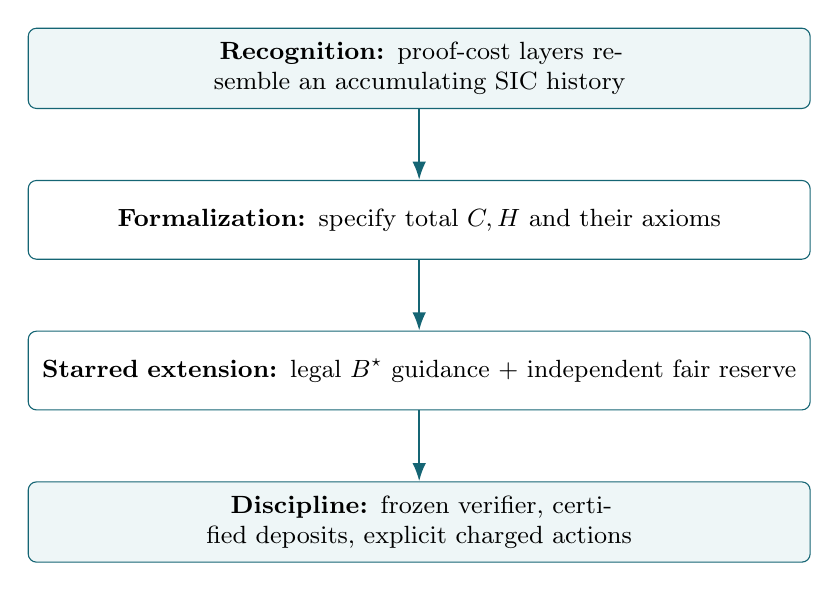
\begin{tikzpicture}[>=Latex,node distance=9mm, every node/.style={font=\small},box/.style={draw=accent,rounded corners=3pt,align=center,minimum height=10mm,text width=0.79\linewidth,inner sep=5pt}]
\node[box,fill=pale] (a) {\textbf{Recognition:} proof-cost layers resemble an accumulating SIC history};
\node[box,below=of a] (b) {\textbf{Formalization:} specify total $C,H$ and their axioms};
\node[box,below=of b] (c) {\textbf{Starred extension:} legal $B^{\star}$ guidance + independent fair reserve};
\node[box,fill=pale,below=of c] (d) {\textbf{Discipline:} frozen verifier, certified deposits, explicit charged actions};
\draw[->,thick,accent] (a)--(b); \draw[->,thick,accent] (b)--(c); \draw[->,thick,accent] (c)--(d);
\end{tikzpicture}
\end{center}

\section{The recursive interrogation}
Each pass asks the original question again at a more demanding level. The pass is successful only if it contributes a distinction not already secured by the previous answer.

\qline{0}{What exactly was first noticed?}
The bounded family $(S_b,b)$ could be viewed as a sequence of growing knowledge states. This answers the \emph{recognition} question. Yet the answer has not explained why that family was eligible for the SIC comparison.

\qline{1}{What made the comparison more than a metaphor?}
The sets are ordered by a meaningful parameter $b$ and are nested: $S_b\subseteq S_{b+1}$. Their union recovers the theorems of the chosen system under the proof assumptions. Thus the analogy uses a definable chronology rather than a verbal resemblance. But a chronology is still only an observation, not a transition system.

\qline{2}{Was the observed pair already the SIC?}
No. It suggested one. The missing item was the formal pair of total state and halt maps, including initialization, persistence, and stopping conventions. This was a close structural identification in need of formal completion, not an erroneous mathematical picture. The source's embedding is the bridge from \emph{SIC-shaped observations} to a \emph{specified SIC}. The origin account must not erase that bridge.

\qline{3}{Did exact addressing create the discovery?}
Exact addressing $D$ made it possible to carry theorem layers as reversible addresses, with no conflation of distinct formulas. It preserved the structure used in the recognition. But an address is a coordinate for something; it neither proves the theorem nor predicts the work needed to find the proof. The discovery is about the structural interpretation of a filtration, not a magic property of an encoding.

\qline{4}{When did a SIC become a proposed prover?}
When the question changed from ``Which theorems have proofs below cost $b$?'' to ``Which legal search step should be attempted to certify this target?'' This adds an objective, an action space, and an operational schedule. Merely naming a SIC does not confer goal-directed discovery.

\qline{5}{Where does the star enter?}
The starred design adds board-guided control: the distinguished GBG+ participant $P_0=B^{\star}$ authorizes a heuristic proving channel while legal moves remain confined to declared transitions. The star denotes a controlled extension, not a claim that the original filtration itself chose proofs.

\qline{6}{Why is control not enough?}
A guide can be mistaken, idle, or indefinitely stalled. The proposed independent reserve systematically enumerates proof candidates. Under a fair schedule, if a finite valid proof of the target exists, the reserve eventually submits one. This protects \emph{positive completeness} but proves neither quick discovery nor termination when no proof exists.

\qline{7}{What converts a search claim into knowledge?}
Only the frozen checker can admit a new consequence. Proposals, addresses, heuristics, and conjectures remain distinct from accepted certificates. The initial BANK stays frozen; later discoveries inhabit an explicitly provisional, verifier-accepted ledger. This explains why the process has an epistemic boundary rather than simply a list of guesses.

\qline{8}{Did proof cost become search time?}
No. At least four quantities must remain distinct: the cost of the final proof, the minimum proof horizon $h(A)$, the charged work expended while looking for the proof, and the first SIC stage at which the target appears. Equating these without a construction would turn the original insight into an unsupported efficiency theorem.

\qline{9}{Was the new system thereby shown universally faster?}
No. The repaired manuscript studies a specific finite Horn-tree family and reports model-specific accepted traces; it also records an ordinary target-aware comparator that may do better than the proposed guide on that family. That bounded demonstration is not a general ATP superiority result or a Metamath/Lean/Coq certification.

\qline{10}{Was $\Ms$ therefore ``found'' or ``made''?}
Both verbs have defensible but different referents. The \emph{pattern} was found by recognizing a familiar SIC structure in an existing proof-cost hierarchy. The \emph{starred architecture} was subsequently made by adding operational states, legal board control, scheduling, proof verification, and accounting. ``Found'' must not suggest that a finished, hidden general-purpose engine was waiting inside the formula for $S_b$.

\qline{11}{What, then, is the irreducible causal account?}
A change of viewpoint produced a formal obligation: if proof-cost layers look like computational history, specify the SIC maps; if the SIC is to search, specify legal choices; if choices can fail, retain fair proof enumeration; if results are to count as knowledge, check them; if efficiency is asserted, measure charged work independently. That chain is how an identification became a construction proposal.

\qline{12}{What new distinction would another identical question force us to add?}
Within the scope of the origin question, none. One may ask for further historical transcripts, new experiments, or a completed implementation, but those are \emph{new evidentiary or engineering tasks}, not a missing logical distinction in the answer about how the idea was identified. The question can now return its own answer unchanged.

\section{Constructing the rhetorical fixed point}
Let $Q$ abbreviate the governing question. Let $E_j$ be an answer that has survived $j$ explanatory passes, and let $\Delta_Q(E_j)$ be the set of \emph{new, question-relevant distinctions} exposed by challenging $E_j$ again. Here $j$ counts rhetorical passes, whereas $n$ in $S_n$ counts proof-cost horizons. An informal elaboration operator is
\begin{equation}\label{eq:operator}
\mathfrak R_Q(E_j)=\operatorname{Normalize}\bigl(E_j\cup\Delta_Q(E_j)\bigr),
\qquad E_{j+1}=\mathfrak R_Q(E_j).
\end{equation}
Normalization removes repetition while preserving the distinctions. For this inquiry we choose the following finite explanatory vocabulary:
\[
\mathcal I=\{\text{recognition, SIC specification, board control,}\
\text{verifier, fairness, costs, evidence boundary}\}.
\]
A \emph{rhetorical fixed point relative to $\mathcal I$} is reached when asking $Q$ again yields no new member of $\mathcal I$ and no reclassification of an existing member:
\begin{equation}\label{eq:fixed}
\boxed{\Delta_Q(E_{\infty})=\varnothing\pmod{\mathcal I},\qquad
\mathfrak R_Q(E_{\infty})\equiv_{\mathcal I}E_{\infty}.}
\end{equation}
Here $\equiv_{\mathcal I}$ means equivalent as an explanation of the origin across the chosen distinctions, \emph{not} literally identical wording. Equation~\eqref{eq:fixed} is a declared rhetorical stopping rule. No mathematical fixed-point theorem establishes that every question, every elaboration policy, or every possible historical record must stabilize.

The stopping rule also exposes what would falsify a premature stop. If a response says only ``$(S_b,b)$ is a SIC,'' pass 2 adds a material correction. If it says ``the SIC is a fast ATP,'' passes 4, 8, and 9 add material corrections. If it says ``the star is the board,'' passes 6 and 7 explain why a board policy and a verifier-gated reserve are also needed. Those are actual increases in explanatory content, not ornamental paraphrases.

\section{The answer that returns to itself}
\vspace{2pt}
\noindent\fcolorbox{accent}{pale}{\parbox{\dimexpr\linewidth-2\fboxsep-2\fboxrule\relax}{\vspace{7pt}
\textbf{Rhetorical fixed point $E_{\infty}$}\par\medskip
\emph{$M^{\star}$ was identified when a filtration of theorems by minimum certified proof cost was recognized as the possible history of a Simulated Intelligent Computer. It was not found as a complete prover inside that filtration. The recognition required formal SIC state and halt maps; the starred construction then added legally authorized board guidance, an independent fair search reserve, frozen verifier-gated certification, and explicit cost accounting. Thus the discovery was a recognition of structure, and $M^{\star}$ was the disciplined attempt to turn that structure into a target-directed proof-search process. Its general-purpose implementation and general efficiency remain separate questions.}\par\vspace{7pt}}}

Now ask again: \emph{Does this address how $M^{\star}$ was identified and found?}

\textbf{Yes}, if ``identified'' means the structural SIC recognition and ``found'' means the constructive path from that recognition to the proposed $\Ms$ architecture. \textbf{No}, if ``found'' is made to mean that the general ATP was already completed, independently certified, or proved universally efficient. The answer itself makes that distinction, so another identical challenge changes nothing relevant to the origin account.

This is the rhetorical return:
\begin{center}
\large\itshape
The question asked where $M^{\star}$ came from.\\
The answer distinguished the seeing from the building.\\
Asked again, the answer is still that distinction.
\end{center}

\section{Scope, provenance, and remaining work}
The inquiry relies on the user's recalled initiating insight and on the repaired $M^{\star}$ research manuscript. That manuscript makes the key formal correction about $(S_b,b)$ and distinguishes a computable SIC specification under explicit assumptions from an independently deployed general ATP. The present note reconstructs a conceptual genealogy; it cannot independently timestamp every conversational step in the original discovery. Version 0.2 adds explicit definitions for the symbols, disambiguates proof-cost $n$ from rhetorical iteration $j$, and records the author's clarification that the initial SIC observation was structurally close but formally incomplete.

To advance beyond this rhetorical fixed point would require an additional goal: e.g., an authenticated chronological transcript of the discovery, a mechanized proof of the SIC axioms in a chosen formal system, a reproducible general-purpose $\Ms$ implementation, or comparative resource measurements. Each would legitimately restart inquiry, but with a new question.

\subsection*{Source note}
\begin{enumerate}[leftmargin=1.7em,itemsep=2pt]
\item Brian Tenneson, \emph{From Proof-Cost SICs to Board-Guided Automated Theorem Proving}, focused Multiarticle joining, repaired research version 0.2, 18 October 2026, especially \S\S 1--5. This is the mathematical baseline for the distinctions made here.
\item \emph{Depths of Induction}, v62, SIC definition and target-first-hit construction, as attributed in source 1.
\item \emph{Universal Proof-Horizon Operator}, audited v1.2; and \emph{GBG and GBG+ Formal Foundations} 004, as attributed in source 1.
\item User--assistant dialogue, 18 October 2026: the question about how $M^{\star}$ was born, the recognition of proof-cost layers as SIC-shaped, and the request to elaborate recursively to a rhetorical fixed point. This note is a synthesis rather than a verbatim transcript.
\end{enumerate}
\vspace{4pt}
{\small\color{muted}\textbf{Version designation:} 0.2, notation-explicit explanatory note, revising 0.1. No claim of an executed new proof-search experiment, a new six-agent federation, a formal certification receipt, or publication to the public research website is made.}
\end{document}
